\documentclass[11pt]{article}
\usepackage[margin=1in]{geometry}
\usepackage{amsmath, amssymb}
\usepackage{graphicx}
\usepackage{tikz}
\usepackage{pgfplots}
\pgfplotsset{compat=1.18}
\usepackage{enumitem}
\usepackage{tcolorbox}
\usepackage{fancyhdr}
\usepackage{siunitx}
\usepackage{cancel}

\tcbuselibrary{breakable}

\newtcolorbox{answerbox}{
  colback=white,
  colframe=black,
  boxrule=1.5pt,
  arc=0pt,
  left=4pt, right=4pt, top=4pt, bottom=4pt,
  breakable
}

\setlength{\headheight}{14pt}
\pagestyle{fancy}
\fancyhf{}
\lhead{EE133 -- Solid-State Electronics}
\chead{Midterm}
\rhead{Winter 2026}
\cfoot{\thepage}

\setlength{\parindent}{0pt}
\setlength{\parskip}{6pt}

\begin{document}

\begin{center}
  {\LARGE \textbf{EE133 Solid-State Electronics -- Midterm}} \\[6pt]
  {\large Winter 2026} \\[6pt]
  \textbf{Name:} Kaushik Vada
\end{center}

\vspace{4pt}
\textbf{Given Constants:}
\begin{itemize}[nosep]
  \item $n_i = 10^{10}\;\text{cm}^{-3}$ at $T = 300\;\text{K}$
  \item $E_G = 1.12\;\text{eV}$ (Si), $\epsilon_s = 11.9\,\epsilon_0$
  \item $kT = 0.026\;\text{eV}$ at $T = 300\;\text{K}$, $q = 1.602 \times 10^{-19}\;\text{C}$
  \item $\epsilon_0 = 8.854 \times 10^{-14}\;\text{F/cm}$, $m_0 = 9.11 \times 10^{-31}\;\text{kg}$
\end{itemize}

\hrule
\vspace{8pt}

%% ========== PROBLEM 1 ==========
\section*{Problem 1 -- Miller Indices of the x-y Plane}

\textbf{(a) (10 pts) What are the Miller indices of the x-y plane?}

The x-y plane is perpendicular to the z-axis. It has intercepts:
\[
  x \to \infty, \quad y \to \infty, \quad z \to 1
\]
Taking the reciprocals:
\[
  \frac{1}{\infty} = 0, \quad \frac{1}{\infty} = 0, \quad \frac{1}{1} = 1
\]

\begin{answerbox}
  The Miller indices of the x-y plane are \textbf{(001)}.
\end{answerbox}

\textbf{(b) (10 pts) List all of the planes equivalent to the x-y plane.}

The family of planes equivalent to (001) consists of all planes perpendicular to one of the three cubic axes. These are:

\begin{answerbox}
  $(001)$, $(010)$, $(100)$, $(00\bar{1})$, $(0\bar{1}0)$, $(\bar{1}00)$
\end{answerbox}

\textbf{(c) (10 pts) Use the correct notation to indicate this full set of equivalent planes.}

\begin{answerbox}
  The full set of equivalent planes is denoted $\{001\}$ (curly braces notation).
\end{answerbox}

\newpage

%% ========== PROBLEM 2 ==========
\section*{Problem 2 -- Miller Indices from the Diagram}

\textbf{(10 pts) What are the Miller indices of the plane at right?}

From the diagram, the plane intercepts the axes at:
\[
  x = 3, \quad y = 4, \quad z = 5
\]
Taking reciprocals:
\[
  \frac{1}{3},\quad \frac{1}{4},\quad \frac{1}{5}
\]
Multiplying through by 60 (the LCM of 3, 4, 5) to get the smallest integers:
\[
  20,\quad 15,\quad 12
\]

\begin{answerbox}
  The Miller indices are \textbf{(20\;15\;12)}.
\end{answerbox}

\newpage

%% ========== PROBLEM 3 ==========
\section*{Problem 3 -- Boron-Doped Silicon}

Si is B-doped at $N_A = 10^{17}\;\text{cm}^{-3}$, $T = 300\;\text{K}$.

\textbf{(a) (10 pts) Determine the electron density.}

Boron is a p-type (acceptor) dopant. Since $N_A = 10^{17} \gg n_i = 10^{10}$, we can assume complete ionization and charge neutrality gives $p \approx N_A = 10^{17}\;\text{cm}^{-3}$.

Using the mass-action law:
\[
  n = \frac{n_i^2}{p} = \frac{(10^{10})^2}{10^{17}} = \frac{10^{20}}{10^{17}}
\]

\begin{answerbox}
  $n = 10^{3}\;\text{cm}^{-3}$
\end{answerbox}

\textbf{(b) (10 pts) Determine the hole density.}

Since $N_A \gg n_i$:

\begin{answerbox}
  $p \approx N_A = 10^{17}\;\text{cm}^{-3}$
\end{answerbox}

\textbf{(c) (10 pts) Which best describes the material: (i) intrinsic or (ii) extrinsic? Why?}

\begin{answerbox}
  \textbf{(ii) Extrinsic.} The material is extrinsic because the dopant concentration $N_A = 10^{17}\;\text{cm}^{-3}$ is many orders of magnitude larger than the intrinsic carrier concentration $n_i = 10^{10}\;\text{cm}^{-3}$. The carrier concentrations are dominated by the Boron doping, not by thermal generation, so $p \gg n$.
\end{answerbox}

\textbf{(d) (20 pts) What is the value (in eV) of $(E_i - E_F)$?}

For p-type material, $E_F$ lies below $E_i$. We use:
\[
  p = n_i \exp\!\left(\frac{E_i - E_F}{kT}\right)
\]
Solving for $E_i - E_F$:
\[
  E_i - E_F = kT \ln\!\left(\frac{p}{n_i}\right)
    = 0.026\;\text{eV} \times \ln\!\left(\frac{10^{17}}{10^{10}}\right)
    = 0.026 \times \ln(10^{7})
\]
\[
  = 0.026 \times 7 \times \ln(10)
  = 0.026 \times 7 \times 2.3026
  = 0.026 \times 16.118
\]

\begin{answerbox}
  $E_i - E_F = 0.419\;\text{eV}$

  Since this is positive, $E_F$ is 0.419 eV below $E_i$, consistent with p-type material.
\end{answerbox}

\newpage

%% ========== PROBLEM 4 ==========
\section*{Problem 4 -- Largest Intrinsic Carrier Concentration}

\textbf{(10 pts) At room temperature, which semiconductor has the largest intrinsic carrier concentration?}

The intrinsic carrier concentration is given by:
\[
  n_i \propto \exp\!\left(-\frac{E_G}{2kT}\right)
\]
A smaller bandgap $E_G$ leads to a larger $n_i$ because the exponential becomes less negative. Comparing the options:
\begin{itemize}[nosep]
  \item (a) Si: $E_G = 1.1\;\text{eV}$
  \item (b) Ge: $E_G = 0.7\;\text{eV}$
  \item (c) GaAs: $E_G = 1.4\;\text{eV}$
  \item (d) InAs: $E_G = 0.35\;\text{eV}$
  \item (e) InSb: $E_G = 0.17\;\text{eV}$
\end{itemize}

\begin{answerbox}
  \textbf{(e) InSb} ($E_G = 0.17\;\text{eV}$) has the largest intrinsic carrier concentration because it has the smallest bandgap. Since $n_i \propto \exp(-E_G / 2kT)$, the smallest $E_G$ produces the largest exponential factor, thus the highest $n_i$.
\end{answerbox}

\newpage

%% ========== PROBLEM 5 ==========
\section*{Problem 5 -- Highest Electron Mobility}

\textbf{(10 pts) At room temperature, which semiconductor has the highest electron mobility?}

All three choices are Si at $T = 300\;\text{K}$, but with different donor concentrations:
\begin{itemize}[nosep]
  \item (a) $N_D = 10^{14}\;\text{cm}^{-3}$
  \item (b) $N_D = 10^{17}\;\text{cm}^{-3}$
  \item (c) $N_D = 10^{18}\;\text{cm}^{-3}$
\end{itemize}

Mobility is affected by both lattice scattering and ionized impurity scattering. As the doping concentration increases, there are more ionized impurities, which increases ionized impurity scattering and decreases mobility. At $N_D = 10^{14}\;\text{cm}^{-3}$, the doping is low enough that lattice scattering dominates and mobility is near its maximum value.

\begin{answerbox}
  \textbf{(a) Si with $N_D = 10^{14}\;\text{cm}^{-3}$} has the highest electron mobility. Lower doping means fewer ionized impurity scattering centers, so the mobility is highest. As $N_D$ increases, ionized impurity scattering reduces $\mu_n$.
\end{answerbox}

\newpage

%% ========== PROBLEM 6 ==========
\section*{Problem 6 -- Highest Conductivity}

\textbf{(10 pts) Which of the above (from Q5) has the highest conductivity?}

Conductivity for n-type material is:
\[
  \sigma = q \, n \, \mu_n
\]
While option (a) has the highest mobility, option (c) has vastly more carriers. The carrier concentration increases by a factor of $10^4$ from (a) to (c), while mobility decreases by roughly a factor of 2--3 at most. The product $n\mu_n$ is therefore largest for (c).

For (a): $\sigma \approx (1.602\times10^{-19})(10^{14})(\sim 1400) \approx 2.24\times10^{-2}\;\text{S/cm}$

For (c): $\sigma \approx (1.602\times10^{-19})(10^{18})(\sim 250) \approx 40\;\text{S/cm}$

\begin{answerbox}
  \textbf{(c) Si with $N_D = 10^{18}\;\text{cm}^{-3}$} has the highest conductivity. Although its mobility is lower, the much higher carrier concentration dominates since $\sigma = qn\mu_n$, and $n$ increases far more than $\mu_n$ decreases.
\end{answerbox}

\newpage

%% ========== PROBLEM 7 ==========
\section*{Problem 7 -- Band Diagram Analysis}

From the band diagram: $E_C$, $E_V$, $E_i$, and $E_F$ are all shown. The bands slope downward from left to right (i.e., $E_C$ and $E_V$ decrease with increasing $x$). Also, $E_{Fn}$ and $E_{Fp}$ are \emph{not} equal -- $E_{Fn}$ is above $E_{Fp}$.

\textbf{(a) (5 pts) It is in equilibrium. T / F}

\begin{answerbox}
  \textbf{False.} The quasi-Fermi levels for electrons ($E_{Fn}$) and holes ($E_{Fp}$) are split (they are not equal). In true thermal equilibrium, there is only one Fermi level, so the system is \emph{not} in equilibrium.
\end{answerbox}

\textbf{(b) (5 pts) The electric field is pointing in which direction?}

The electric field is related to the band bending by:
\[
  \mathcal{E} = \frac{1}{q}\frac{dE_C}{dx}
\]
Since $E_C$ decreases from left to right, $dE_C/dx < 0$, so $\mathcal{E} < 0$, meaning the field points in the negative $x$-direction (to the left).

\begin{answerbox}
  \textbf{(i) Left.} The bands slope downward to the right ($dE_C/dx < 0$), so the electric field points to the left.
\end{answerbox}

\textbf{(c) (5 pts) There is an electron drift current flowing\ldots}

Electron drift current (conventional current) is:
\[
  J_{n,\text{drift}} = qn\mu_n \mathcal{E}
\]
Since $q > 0$, $n > 0$, $\mu_n > 0$, and $\mathcal{E}$ points to the left, $J_{n,\text{drift}}$ flows to the left.

\begin{answerbox}
  \textbf{(i) To the left.}
\end{answerbox}

\textbf{(d) (5 pts) There is an electron diffusion current flowing\ldots}

From the band diagram, $E_C$ and $E_{Fn}$ decrease at the same rate (they are parallel). This means $E_C - E_{Fn}$ is constant across position. Since $n \propto \exp(-(E_C - E_{Fn})/kT)$, the electron concentration is uniform, so $dn/dx = 0$.
\[
  J_{n,\text{diff}} = qD_n \frac{dn}{dx} = 0
\]

\begin{answerbox}
  \textbf{(iii) Neither, since it is zero.} $E_C$ and $E_{Fn}$ are parallel, so $E_C - E_{Fn}$ is constant, meaning the electron concentration is uniform and there is no diffusion current.
\end{answerbox}

\textbf{(e) (5 pts) There is a hole drift current flowing\ldots}

Hole drift current flows in the same direction as the electric field:
\[
  J_{p,\text{drift}} = qp\mu_p \mathcal{E}
\]
Since $\mathcal{E}$ points to the left:

\begin{answerbox}
  \textbf{(i) To the left.}
\end{answerbox}

\textbf{(f) (5 pts) There is a hole diffusion current flowing\ldots}

Hole concentration depends on $E_{Fp} - E_V$: $p \propto \exp(-(E_{Fp} - E_V)/kT)$. From the diagram, $E_V$ decreases to the right while $E_{Fp}$ is approximately flat, so $E_{Fp} - E_V$ \emph{increases} to the right, meaning $p$ \emph{decreases} to the right. Holes diffuse from high concentration (left) to low concentration (right). The hole diffusion current is:
\[
  J_{p,\text{diff}} = -qD_p \frac{dp}{dx}
\]
Since $dp/dx < 0$ (hole concentration decreases to the right), $J_{p,\text{diff}} = -qD_p(\text{negative}) > 0$, so the current flows to the right.

\begin{answerbox}
  \textbf{(ii) To the right.}
\end{answerbox}

\textbf{(g) (5 pts) The total electron current is flowing\ldots}

The total electron current is proportional to the gradient of the electron quasi-Fermi level:
\[
  J_n = n\mu_n \frac{dE_{Fn}}{dx}
\]
From the diagram, $E_{Fn}$ slopes downward from left to right ($dE_{Fn}/dx < 0$). Therefore:

\begin{answerbox}
  \textbf{(i) To the left.} Since $E_{Fn}$ has a negative slope ($dE_{Fn}/dx < 0$), the total electron current flows in the negative $x$-direction (to the left).
\end{answerbox}

\textbf{(h) (5 pts) The total hole current is flowing\ldots}

Similarly:
\[
  J_p = -p\mu_p \frac{dE_{Fp}}{dx}
\]
From the diagram, $E_{Fp}$ appears approximately flat/constant ($dE_{Fp}/dx \approx 0$).

\begin{answerbox}
  \textbf{(iii) Neither, since it is zero.} $E_{Fp}$ is approximately constant (flat), so the total hole current is approximately zero.
\end{answerbox}

\newpage

%% ========== PROBLEM 8 ==========
\section*{Problem 8 -- Minority Carrier Hole Distributions}

The figure shows two minority carrier hole distributions (excess hole concentration $\delta p_n$ vs.\ position $x$): a solid curve that decays exponentially and a dashed curve that decays linearly (steeper initial slope). Both start at the same $\delta p_n$ value at $x=0$ and decay to zero at $x = W$.

\textbf{(a) (5 pts) Circle the one which results in the largest diffusion current at $x=0$.}

\begin{answerbox}
  The \textbf{solid (exponential) curve} produces the largest diffusion current at $x=0$ because it starts at the higher excess concentration $\delta p_n$ and has the steeper slope (larger $|dp/dx|$) at $x=0$.
\end{answerbox}

\textbf{(b) (5 pts) Explain using an equation.}

The hole diffusion current is:
\[
  J_{p,\text{diff}} = -qD_p \frac{dp}{dx}\bigg|_{x=0}
\]
The magnitude of the diffusion current depends on $|dp/dx|$ at $x=0$. The solid curve begins at the higher initial excess concentration ($\delta p_n > \Delta p_n$) and decays exponentially, giving it a steeper initial slope at $x = 0$:
\[
  \left|\frac{dp}{dx}\bigg|_{x=0,\;\text{solid}}\right| > \left|\frac{dp}{dx}\bigg|_{x=0,\;\text{dashed}}\right|
\]

\begin{answerbox}
  Since $|J_p| = qD_p |dp/dx|$, the solid curve's steeper slope at $x=0$ gives a larger diffusion current.
\end{answerbox}

\textbf{(c) (5 pts) What direction is the hole diffusion current flowing?}

Both curves show $\delta p_n$ decreasing with increasing $x$ (i.e., $dp/dx < 0$). Holes diffuse from high to low concentration, meaning holes move in the $+x$ direction. Since holes are positive carriers, the diffusion current flows in the same direction as the hole flow.

\begin{answerbox}
  The hole diffusion current is flowing in the \textbf{positive $x$-direction} (to the right), from high concentration toward low concentration.
\end{answerbox}

\textbf{(d) (10 pts) Comparing the solid curve to the dashed curve, what physical mechanism is present or absent?}

The four solutions of the minority carrier diffusion equation (MCDE) include terms with $\exp(-x/L_p)$, $\exp(+x/L_p)$, $\sinh$, and $\cosh$ forms, depending on boundary conditions.

The solid curve shows an exponential decay $\delta p_n \propto \exp(-x/L_p)$, which is the solution when recombination is present (the minority carrier lifetime $\tau_p$ is finite). The diffusion length $L_p = \sqrt{D_p \tau_p}$ governs the decay.

The dashed curve is linear, which is the solution when there is \emph{no recombination} ($\tau_p \to \infty$, or $L_p \to \infty$). In this limit, the MCDE reduces to $d^2(\delta p)/dx^2 = 0$, giving a linear profile.

\begin{answerbox}
  \textbf{Recombination} is the physical mechanism that differs between the two curves. The solid (exponential) curve has recombination present ($\tau_p$ is finite), causing the excess carriers to decay exponentially with diffusion length $L_p = \sqrt{D_p \tau_p}$. The dashed (linear) curve represents the case where recombination is \emph{absent} ($\tau_p \to \infty$), so the MCDE simplifies to $d^2(\delta p)/dx^2 = 0$, yielding a straight-line profile.
\end{answerbox}

\newpage

%% ========== PROBLEM 9 ==========
\section*{Problem 9 -- Resistor Bar of p-type Si}

Given: $L = 10\;\mu\text{m}$, $W = 1\;\mu\text{m}$, $t = 0.1\;\mu\text{m}$, $N_A = 10^{18}\;\text{cm}^{-3}$, $\mu_p = 642.2\;\text{cm}^2/\text{Vs}$, $m_p^* = 0.4\,m_0$, $J = 1 \times 10^5\;\text{A/cm}^2$.

First, convert dimensions: $L = 10 \times 10^{-4}\;\text{cm} = 10^{-3}\;\text{cm}$, $W = 10^{-4}\;\text{cm}$, $t = 10^{-5}\;\text{cm}$.

The conductivity is:
\[
  \sigma = q \, N_A \, \mu_p = (1.602 \times 10^{-19})(10^{18})(642.2) = 0.1602 \times 642.2 = 102.88\;\text{S/cm}
\]
The resistivity is:
\[
  \rho = \frac{1}{\sigma} = \frac{1}{102.88} = 9.72 \times 10^{-3}\;\Omega\!\cdot\!\text{cm}
\]

\textbf{(a) (10 pts) What is the sheet resistance?}

\[
  R_{\text{sh}} = \frac{\rho}{t}
  = \frac{9.72 \times 10^{-3}\;\Omega\!\cdot\!\text{cm}}{10^{-5}\;\text{cm}}
\]

\begin{answerbox}
  $R_{\text{sh}} = 972\;\Omega/\square$
\end{answerbox}

\textbf{(b) (10 pts) What is the resistance?}

Using $R = \rho L / A$ where $A = W \times t$:
\[
  A = W \times t = (10^{-4})(10^{-5}) = 10^{-9}\;\text{cm}^2
\]
\[
  R = \frac{\rho \, L}{A}
  = \frac{(9.72 \times 10^{-3})(10^{-3})}{10^{-9}}
  = \frac{9.72 \times 10^{-6}}{10^{-9}}
\]

Or equivalently, $R = R_{\text{sh}} \times \frac{L}{W} = 972 \times \frac{10}{1}$:

\begin{answerbox}
  $R = 9720\;\Omega \approx 9.72\;\text{k}\Omega$
\end{answerbox}

\textbf{(c) (20 pts) What is the average drift velocity of a hole (cm/s)?}

The current density is related to drift velocity by:
\[
  J = qp\,v_d
\]
Since $p \approx N_A = 10^{18}\;\text{cm}^{-3}$:
\[
  v_d = \frac{J}{qp} = \frac{1 \times 10^5}{(1.602 \times 10^{-19})(10^{18})}
  = \frac{10^5}{0.1602}
\]

\begin{answerbox}
  $v_d = 6.24 \times 10^{5}\;\text{cm/s}$
\end{answerbox}

\textbf{(d) (20 pts) For a hole, what is the average time between collisions (average scattering time)?}

The mobility is related to the scattering time by:
\[
  \mu_p = \frac{q\,\tau_{\text{sc}}}{m_p^*} \quad \Longrightarrow \quad
  \tau_{\text{sc}} = \frac{\mu_p \, m_p^*}{q}
\]
First, $m_p^* = 0.4\,m_0 = 0.4 \times 9.11 \times 10^{-31} = 3.644 \times 10^{-31}\;\text{kg}$.

Converting $\mu_p$ to SI units: $642.2\;\text{cm}^2/\text{Vs} = 642.2 \times 10^{-4}\;\text{m}^2/\text{Vs} = 6.422 \times 10^{-2}\;\text{m}^2/\text{Vs}$.

\[
  \tau_{\text{sc}} = \frac{(6.422 \times 10^{-2})(3.644 \times 10^{-31})}{1.602 \times 10^{-19}}
  = \frac{2.340 \times 10^{-32}}{1.602 \times 10^{-19}}
\]

\begin{answerbox}
  $\tau_{\text{sc}} = 1.46 \times 10^{-13}\;\text{s}$
\end{answerbox}

\newpage

%% ========== PROBLEM 10 ==========
\section*{Problem 10 -- Illuminated Semiconductor Bar}

Given: $N_D = 10^{16}\;\text{cm}^{-3}$, $p(x=0) = 10^{12}\;\text{cm}^{-3}$, $n_i = 10^{10}\;\text{cm}^{-3}$, $\mu_n = 1154\;\text{cm}^2/\text{Vs}$, $\mu_p = 384.6\;\text{cm}^2/\text{Vs}$, $\tau_n = \tau_p = 0.1\;\mu\text{s} = 10^{-7}\;\text{s}$, $T = 300\;\text{K}$.

First, find equilibrium values. Since $N_D = 10^{16} \gg n_i$:
\[
  n_0 = N_D = 10^{16}\;\text{cm}^{-3}, \qquad p_0 = \frac{n_i^2}{N_D} = \frac{10^{20}}{10^{16}} = 10^4\;\text{cm}^{-3}
\]

The excess minority carrier concentration at $x = 0$:
\[
  \delta p(0) = p(0) - p_0 = 10^{12} - 10^4 \approx 10^{12}\;\text{cm}^{-3}
\]

Diffusion coefficient for holes:
\[
  D_p = \frac{kT}{q}\mu_p = (0.026)(384.6) = 9.9996 \approx 10\;\text{cm}^2/\text{s}
\]

Diffusion length for holes:
\[
  L_p = \sqrt{D_p \tau_p} = \sqrt{(10)(10^{-7})} = \sqrt{10^{-6}} = 10^{-3}\;\text{cm} = 10\;\mu\text{m}
\]

\textbf{(a) (10 pts) What is the optical generation rate $g_{\text{op}}$ in (cm$^{-3}$\,s$^{-1}$)?}

At steady state, at $x = 0$ the generation must sustain the excess carriers. The excess concentration satisfies:
\[
  \delta p(0) = g_{\text{op}} \, \tau_p
\]
\[
  g_{\text{op}} = \frac{\delta p(0)}{\tau_p} = \frac{10^{12}}{10^{-7}}
\]

\begin{answerbox}
  $g_{\text{op}} = 10^{19}\;\text{cm}^{-3}\text{s}^{-1}$
\end{answerbox}

\textbf{(b) (10 pts) Are the conditions of low-level injection satisfied? Why or why not?}

Low-level injection requires $\delta p \ll n_0$ (excess minority carriers much less than the majority carrier concentration).

\[
  \delta p(0) = 10^{12}\;\text{cm}^{-3}, \qquad n_0 = N_D = 10^{16}\;\text{cm}^{-3}
\]
\[
  \delta p(0) = 10^{12} \ll 10^{16} = n_0 \qquad \checkmark
\]

\begin{answerbox}
  \textbf{Yes}, low-level injection conditions are satisfied because $\delta p(0) = 10^{12}\;\text{cm}^{-3} \ll n_0 = 10^{16}\;\text{cm}^{-3}$. The excess minority carrier concentration is four orders of magnitude smaller than the majority carrier concentration.
\end{answerbox}

\textbf{(c) (10 pts) Calculate the electron and hole densities at $x = 100\;\mu\text{m}$.}

Since no light penetrates beyond $x = 0$, the excess holes decay exponentially for $x > 0$:
\[
  \delta p(x) = \delta p(0)\,\exp\!\left(-\frac{x}{L_p}\right)
\]
At $x = 100\;\mu\text{m}$:
\[
  \delta p(100\;\mu\text{m}) = 10^{12}\,\exp\!\left(-\frac{100}{10}\right) = 10^{12}\,e^{-10}
\]
\[
  e^{-10} = 4.54 \times 10^{-5}
\]
\[
  \delta p = 10^{12} \times 4.54 \times 10^{-5} = 4.54 \times 10^{7}\;\text{cm}^{-3}
\]

\begin{answerbox}
  At $x = 100\;\mu\text{m}$:
  \[
    p = p_0 + \delta p = 10^4 + 4.54 \times 10^7 \approx 4.54 \times 10^7\;\text{cm}^{-3}
  \]
  \[
    n = n_0 + \delta n = 10^{16} + 4.54 \times 10^7 \approx 10^{16}\;\text{cm}^{-3}
  \]
  (The excess carriers are negligible compared to the majority electron concentration.)
\end{answerbox}

\textbf{(d) (20 pts) Calculate the hole current at $x = 0$.}

Under low-level injection with no electric field in the quasi-neutral region, the minority carrier (hole) current density at $x = 0$ is purely diffusion:
\[
  J_p(x) = -qD_p \frac{d(\delta p)}{dx}
\]
The excess carrier profile is $\delta p(x) = \delta p(0)\,e^{-x/L_p}$, so:
\[
  \frac{d(\delta p)}{dx}\bigg|_{x=0} = -\frac{\delta p(0)}{L_p}
\]
Therefore:
\[
  J_p(0) = -qD_p\left(-\frac{\delta p(0)}{L_p}\right) = \frac{qD_p\,\delta p(0)}{L_p}
\]
\[
  = \frac{(1.602 \times 10^{-19})(10)(10^{12})}{10^{-3}}
  = \frac{1.602 \times 10^{-6}}{10^{-3}}
\]

\begin{answerbox}
  $J_p(0) \approx 1.6 \times 10^{-3}\;\text{A/cm}^2 = 1.6\;\text{mA/cm}^2$

  The current flows in the positive $x$-direction (to the right), away from the illuminated surface, since holes diffuse from high concentration at $x=0$ toward lower concentration.
\end{answerbox}

\textbf{(e) (10 pts) If we increase the recombination times, will the hole current increase or decrease? Why?}

If $\tau_p$ increases, then $L_p = \sqrt{D_p \tau_p}$ increases. The current at $x = 0$ is:
\[
  J_p(0) = \frac{qD_p\,\delta p(0)}{L_p} = \frac{qD_p\,\delta p(0)}{\sqrt{D_p\tau_p}} = q\,\delta p(0)\sqrt{\frac{D_p}{\tau_p}}
\]
As $\tau_p$ increases, $\sqrt{D_p/\tau_p}$ \emph{decreases}, so $J_p(0)$ decreases.

\begin{answerbox}
  The hole current will \textbf{decrease}. Increasing the recombination time increases the diffusion length $L_p$, which reduces the concentration gradient $|dp/dx|$ at $x=0$. Since $J_p \propto 1/L_p \propto 1/\sqrt{\tau_p}$, a larger $\tau_p$ means a smaller hole current.
\end{answerbox}

\newpage

%% ========== PROBLEM 11 ==========
\section*{Problem 11 -- Electrostatic Potential and Band Diagram}

From the figure, the electrostatic potential $V(x)$ is:
\begin{itemize}[nosep]
  \item For $x < 0$: $V \approx 0\;\text{V}$ (constant)
  \item For $0 \le x \le 0.5\;\mu\text{m}$: $V$ decreases linearly from $0\;\text{V}$ to $-1\;\text{V}$
  \item For $x > 0.5\;\mu\text{m}$: $V = -1\;\text{V}$ (constant)
\end{itemize}

\textbf{(a) (10 pts) On plot (b), plot the conduction band edge.}

The conduction band edge is related to the electrostatic potential by:
\[
  E_C(x) = E_{C,\text{ref}} - qV(x)
\]
Since $E_C$ is inversely related to $V$: where $V$ goes down, $E_C$ goes up, and vice versa.

From the diagram, plot (b) already has the start of $E_C$ drawn at a constant level for $x < 0$. The conduction band should:
\begin{itemize}[nosep]
  \item For $x < 0$: $E_C$ is constant at a reference level (since $V = 0$)
  \item For $0 \le x \le 0.5$: $E_C$ increases linearly (since $V$ decreases linearly, $-qV$ increases)
  \item For $x > 0.5$: $E_C$ is constant at a higher value (since $V = -1$ V $\Rightarrow$ $E_C = E_{C,\text{ref}} + 1\;\text{eV}$)
\end{itemize}

\begin{answerbox}
  The conduction band edge $E_C$ mirrors the potential $V(x)$ with inverted sign ($E_C = \text{const} - qV$):

  \begin{center}
  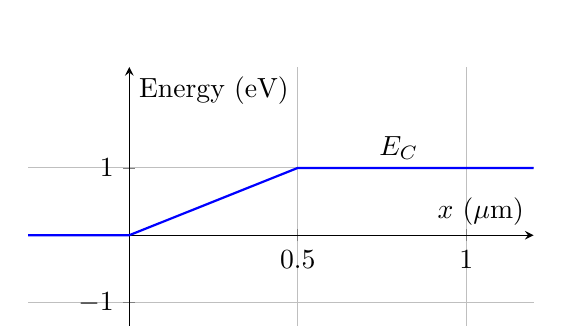
\begin{tikzpicture}
    \begin{axis}[
      width=8cm, height=5cm,
      xlabel={$x$ ($\mu$m)},
      ylabel={Energy (eV)},
      xmin=-0.3, xmax=1.2,
      ymin=-1.5, ymax=2.5,
      axis lines=middle,
      xtick={0, 0.5, 1.0},
      ytick={-1, 0, 1},
      grid=major,
    ]
    \addplot[thick, blue] coordinates {(-0.3,0) (0,0) (0.5,1) (1.0,1) (1.2,1)};
    \node at (axis cs:0.8,1.3) {$E_C$};
    \end{axis}
  \end{tikzpicture}
  \end{center}

  $E_C$ is constant (low) for $x < 0$, increases linearly from $x = 0$ to $x = 0.5\;\mu$m, then is constant (high) for $x > 0.5\;\mu$m.
\end{answerbox}

\textbf{(b) (20 pts) Plot the electric field on plot (c).}

The electric field is:
\[
  \mathcal{E} = -\frac{dV}{dx}
\]
\begin{itemize}[nosep]
  \item For $x < 0$: $V$ is constant, so $\mathcal{E} = 0$
  \item For $0 \le x \le 0.5\;\mu\text{m}$: $V$ decreases linearly from $0$ to $-1$ V over $0.5\;\mu\text{m}$:
    \[
      \frac{dV}{dx} = \frac{-1 - 0}{0.5\;\mu\text{m}} = -2\;\text{V}/\mu\text{m}
    \]
    \[
      \mathcal{E} = -\frac{dV}{dx} = -(-2) = +2\;\text{V}/\mu\text{m}
    \]
  \item For $x > 0.5\;\mu\text{m}$: $V$ is constant, so $\mathcal{E} = 0$
\end{itemize}

\begin{answerbox}
  \begin{center}
  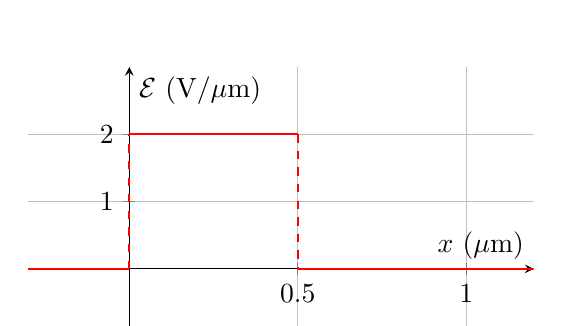
\begin{tikzpicture}
    \begin{axis}[
      width=8cm, height=5cm,
      xlabel={$x$ ($\mu$m)},
      ylabel={$\mathcal{E}$ (V/$\mu$m)},
      xmin=-0.3, xmax=1.2,
      ymin=-1, ymax=3,
      axis lines=middle,
      xtick={0, 0.5, 1.0},
      ytick={0, 1, 2},
      grid=major,
    ]
    \addplot[thick, red] coordinates {(-0.3,0) (0,0)};
    \addplot[thick, red, dashed] coordinates {(0,0) (0,2)};
    \addplot[thick, red] coordinates {(0,2) (0.5,2)};
    \addplot[thick, red, dashed] coordinates {(0.5,2) (0.5,0)};
    \addplot[thick, red] coordinates {(0.5,0) (1.2,0)};
    \end{axis}
  \end{tikzpicture}
  \end{center}

  The electric field is $\mathcal{E} = 0$ for $x < 0$ and $x > 0.5\;\mu$m, and $\mathcal{E} = +2\;\text{V}/\mu\text{m}$ (pointing in the $+x$ direction) for $0 < x < 0.5\;\mu$m.
\end{answerbox}

\newpage

%% ========== PROBLEM 12 ==========
\section*{Problem 12 -- Band Diagram with Applied Voltage}

The band diagram of a uniformly doped n-type semiconductor (flat bands, electrons on $E_C$, holes on $E_V$) is drawn with $V = 0$. A positive voltage $V > 0$ is applied (+ on left, $-$ on right).

\textbf{(a) (10 pts) Sketch the band diagram with $V > 0$.}

With $V > 0$ applied (positive terminal on the left), the potential on the left side is higher. Since $E_C = \text{const} - qV$, higher potential means lower band energy. The bands will tilt such that $E_C$ and $E_V$ are \emph{lower on the left} and \emph{higher on the right} (bands slope upward from left to right).

\begin{answerbox}
  \begin{center}
  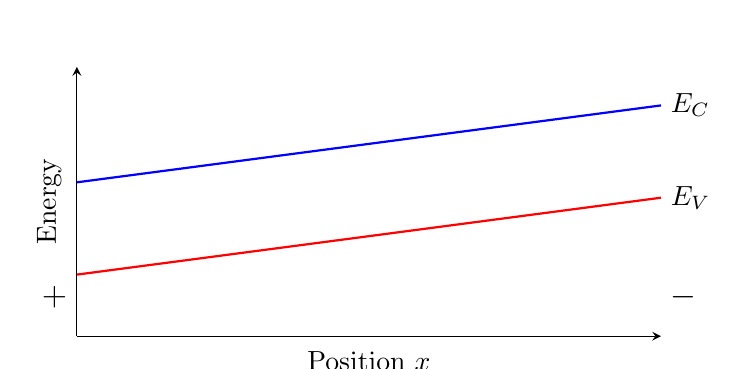
\begin{tikzpicture}
    \begin{axis}[
      width=9cm, height=5cm,
      xlabel={Position $x$},
      ylabel={Energy},
      xmin=0, xmax=5,
      ymin=-0.5, ymax=3,
      axis lines=left,
      xtick=\empty,
      ytick=\empty,
      clip=false,
    ]
    \addplot[thick, blue] coordinates {(0,1.5) (5,2.5)};
    \node[right] at (axis cs:5,2.5) {$E_C$};
    \addplot[thick, red] coordinates {(0,0.3) (5,1.3)};
    \node[right] at (axis cs:5,1.3) {$E_V$};
    \node[left] at (axis cs:0,0) {\large $+$};
    \node[right] at (axis cs:5,0) {\large $-$};
    \end{axis}
  \end{tikzpicture}
  \end{center}

  The bands tilt upward from left ($+$) to right ($-$). $E_C$ and $E_V$ both increase from left to right.
\end{answerbox}

\textbf{(b) (10 pts) Show directions of electron velocities $v_n$ and hole velocities $v_p$.}

The electric field points from high potential to low potential, i.e., from left ($+$) to right ($-$). So $\vec{\mathcal{E}}$ points to the right.

\begin{itemize}
  \item Electrons (negative charge) drift \emph{opposite} to $\vec{\mathcal{E}}$: $v_n$ points to the \textbf{left}.
  \item Holes (positive charge) drift \emph{with} $\vec{\mathcal{E}}$: $v_p$ points to the \textbf{right}.
\end{itemize}

\begin{answerbox}
  $v_n \leftarrow$ (electrons move to the left) \\
  $v_p \rightarrow$ (holes move to the right)
\end{answerbox}

\textbf{(c) (10 pts) Show which way the electric field is pointing.}

\begin{answerbox}
  $\vec{\mathcal{E}} \rightarrow$ The electric field points from the $+$ terminal to the $-$ terminal, i.e., to the \textbf{right}.
\end{answerbox}

\textbf{(d) (10 pts) Show which way the electrical current due to electrons, $J_n$, is flowing.}

Electron drift current (conventional current) is opposite to electron velocity:
\[
  J_n = qn\mu_n\mathcal{E}
\]
Since $\mathcal{E}$ is to the right and $q > 0$, $n > 0$, $\mu_n > 0$:

\begin{answerbox}
  $J_n \rightarrow$ The electron current flows to the \textbf{right} (conventional current is opposite to electron motion).
\end{answerbox}

\textbf{(e) (10 pts) Show which way the electrical current due to holes, $J_p$, is flowing.}

\[
  J_p = qp\mu_p\mathcal{E}
\]
Hole current flows in the same direction as hole velocity (same as $\mathcal{E}$):

\begin{answerbox}
  $J_p \rightarrow$ The hole current flows to the \textbf{right}. Both $J_n$ and $J_p$ flow in the same direction (to the right), so the total conventional current flows to the right.
\end{answerbox}

\end{document}
